\documentclass[10pt]{article}
\usepackage{amsmath}
\usepackage{amssymb}
\usepackage{mathtools}
\usepackage{calc}
\usepackage[margin=1in]{geometry}

\pagestyle{empty}
\begin{document}
\thispagestyle{empty}
\makebox{\hspace{1cm}}
\vspace{-0.5in}
\begin{center}

{\Large \bf PHYS425: In-class worksheet \#1} \\
\end{center}


\vspace{0.5cm}
\begin{tabular}{ll}
Name: & \quad \rule{5in}{0.4pt} \\[0.3cm]
Partners Name: &  \quad \rule{5in}{0.4pt} 
\end{tabular}
\vspace{0.5cm}

\vspace{0.5cm}
This worksheet is to introduce the idea that scalar quantities are easier to work with than vectors. Because we are physicist, we like making all comparisons quantitative. So if possible (Using your phones, or just the wall clock) time youselves with these problems.

\begin{center}
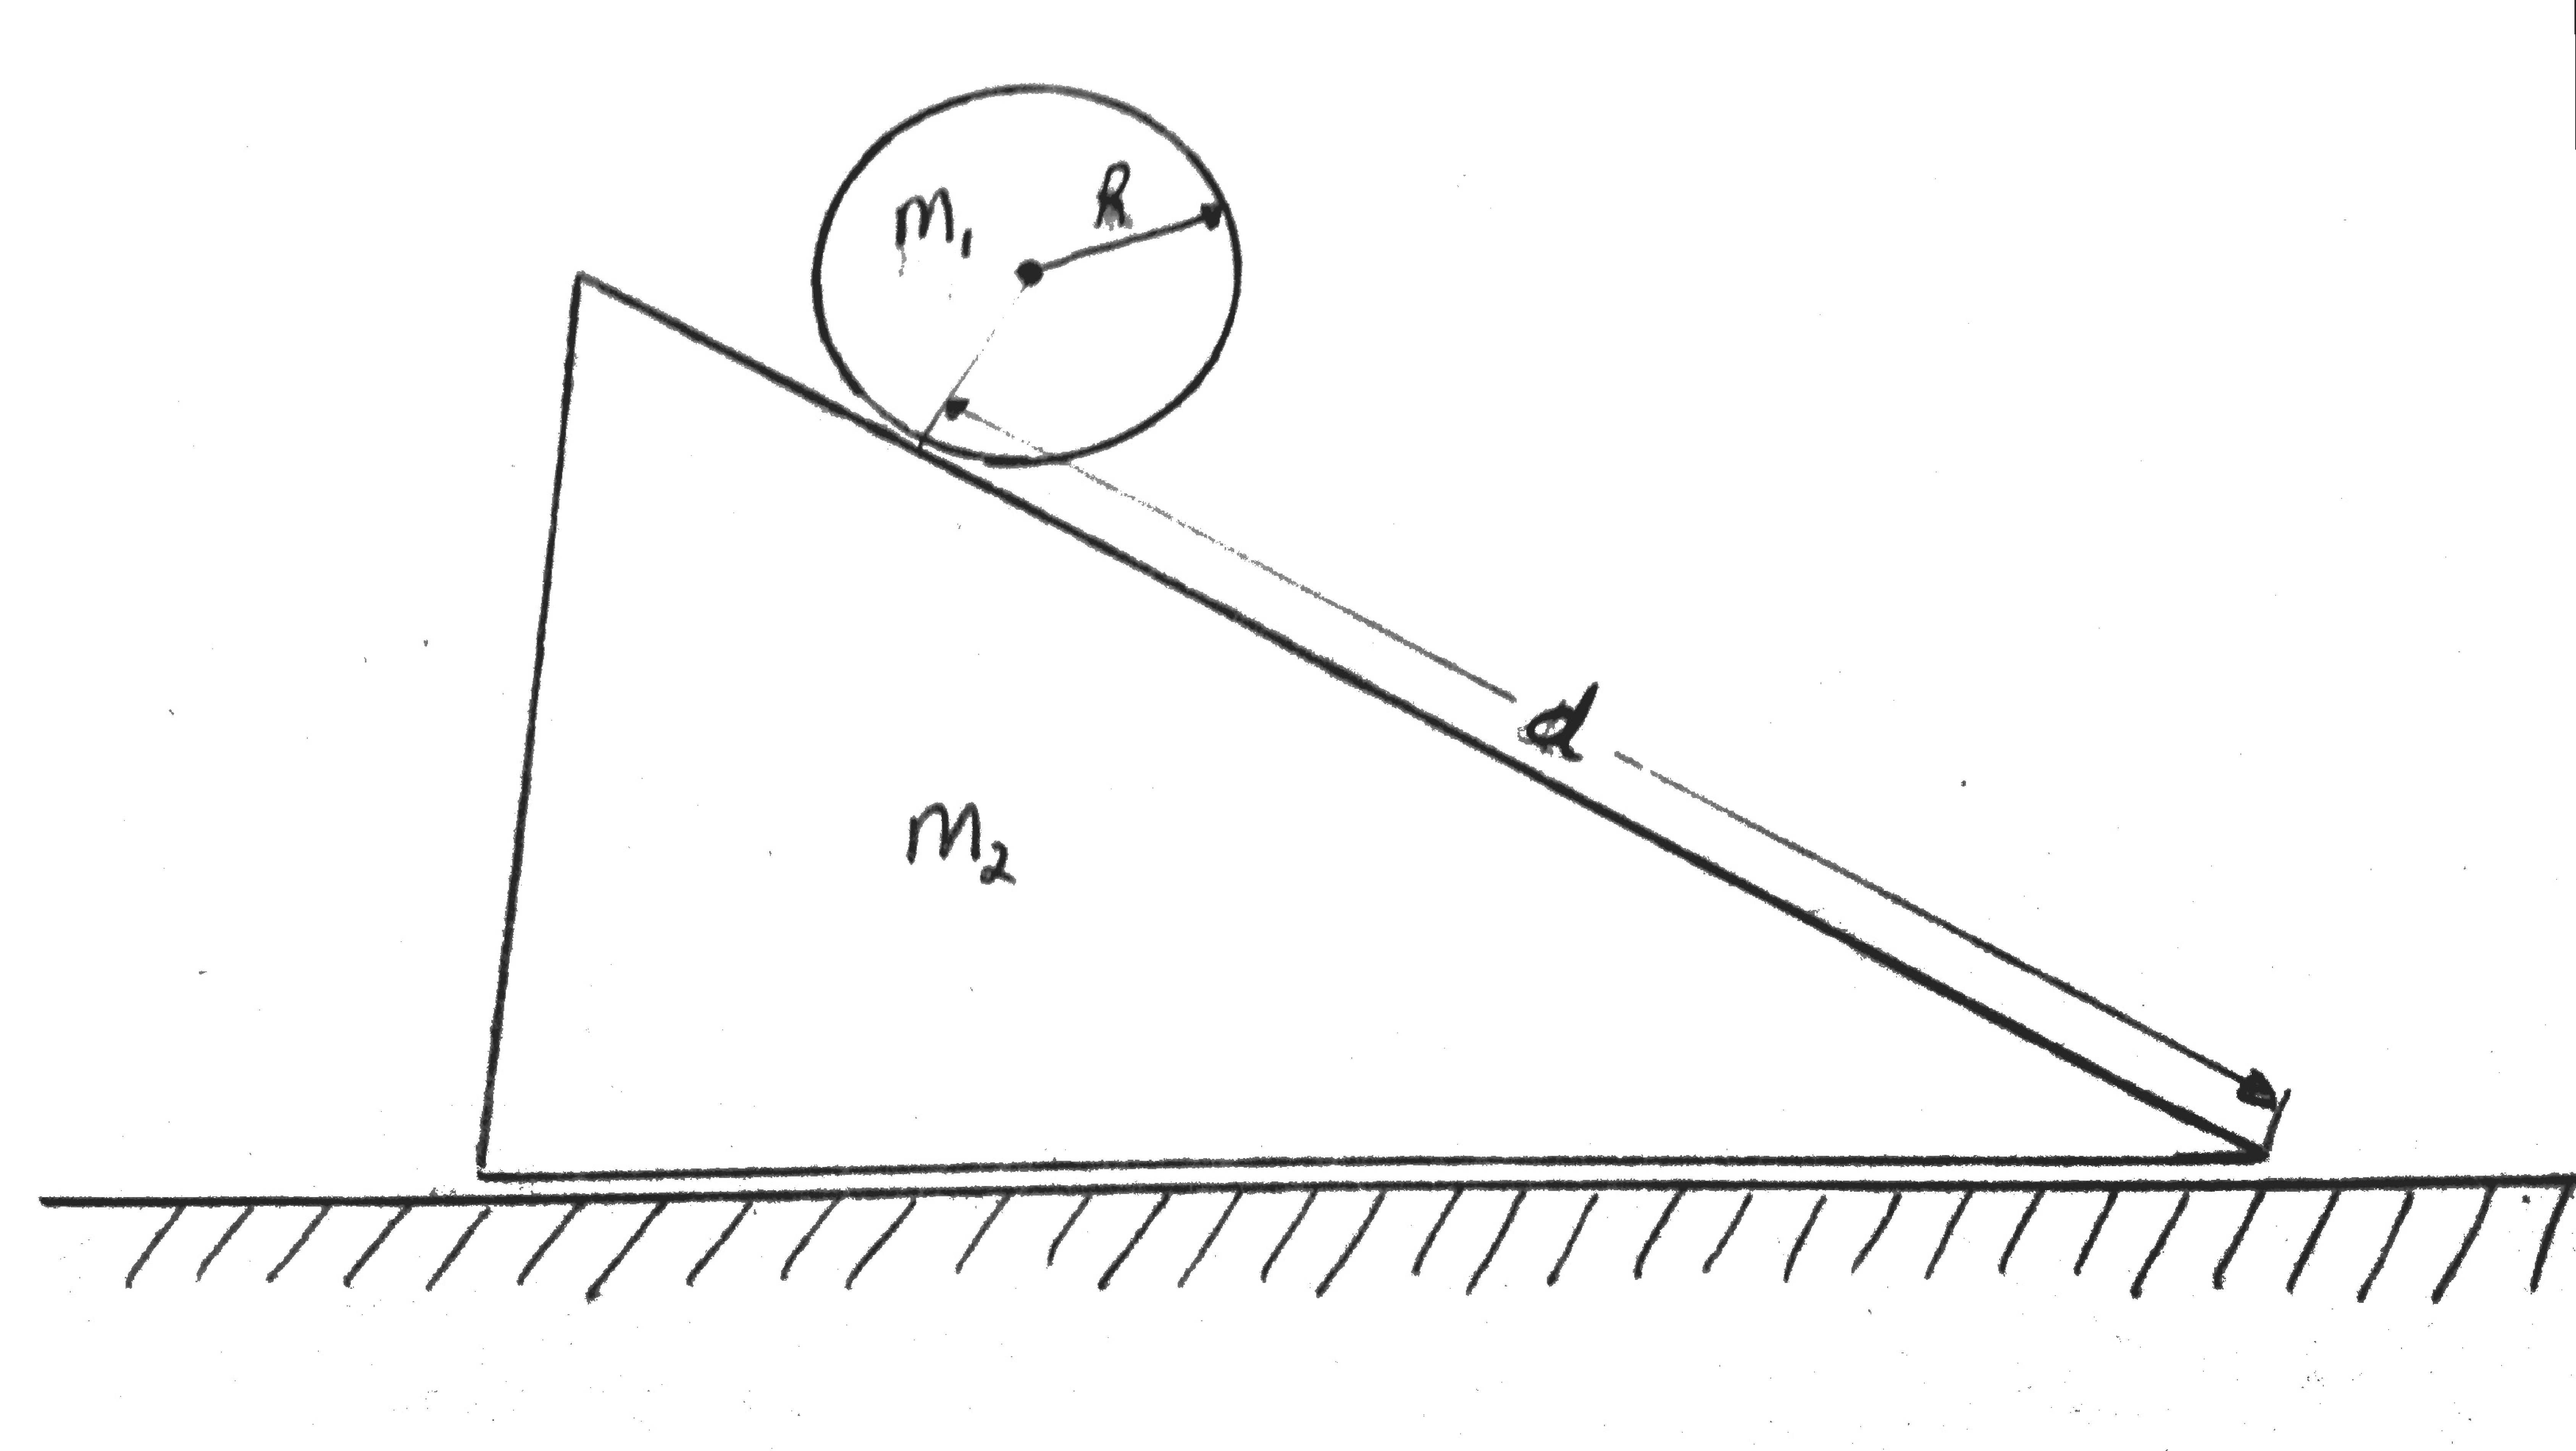
\includegraphics[width=0.6\textwidth]{fig.pdf}
\end{center}

A block of mass $m_1$ is place a distance $d$ up a wedge of mass $m_2$ that makes an angle $\theta$ with the level ground. The block slides without friction upon the wedge, and the wedge slides without friction upon the ground.

\begin{enumerate}
\item We have enough information to find the forces acting upon the block and the wedge. Use Newton's second and third laws find the equations that describe the positions of the block and wedge at some future time $t$. When does the block begin to leave the wedge? (Reminder it is fun to time yourselves with these problems).

\newpage

\item Now use the conservation of energy and momentum to describe the positions of the block and the wedge at some future time $t$. When does the block begin to leave the wedge?

\vspace{7in}

\item If you timed yourself how long did the two problems take?

\end{enumerate}

\end{document}